\chapter{Thiết kế hệ thống}\label{chap2}
\section{Kiến trúc hệ thống}
Nền tảng hạ tầng của hệ thống được thiết kế giúp hướng đến tính ổn định cao và phát triển cho sau này.
Khi hệ thống đạt một số lượng người dùng nhất định, và có thể những người dùng này trải dài khắp nơi thay vì tập trung chủ yếu tại một địa điểm cố định.
Khi đó, việc duy trì một máy chủ vật lý sẽ không còn là lựa chọn tối ưu do sự tốn kém về nhân lực cũng như chi phí phát sinh trong việc bảo trì và nâng cấp cho máy chủ.
Từ đó mô hình kiến trúc của dự án hướng tới triển khai trên môi trường đám mây, tức sử dụng máy chủ của các nhà cung cấp dịch vụ đám mây rải rác ở khắp nơi trên thế giới.
Điều này sẽ giúp giảm đáng kể thời gian cấu hình máy chủ vật lý của hệ thống cũng như thời gian cần phải bỏ ra giúp duy trì và bảo dưỡng do các tác nhân bên ngoài gây nên.

Hình \ref{fig:overall-architecture} dưới đây mô tả kiến trúc tổng quan của nền tảng quản lý quán ăn triển khai trên môi trường đám mây.

\begin{figure}[h]
	\centering
	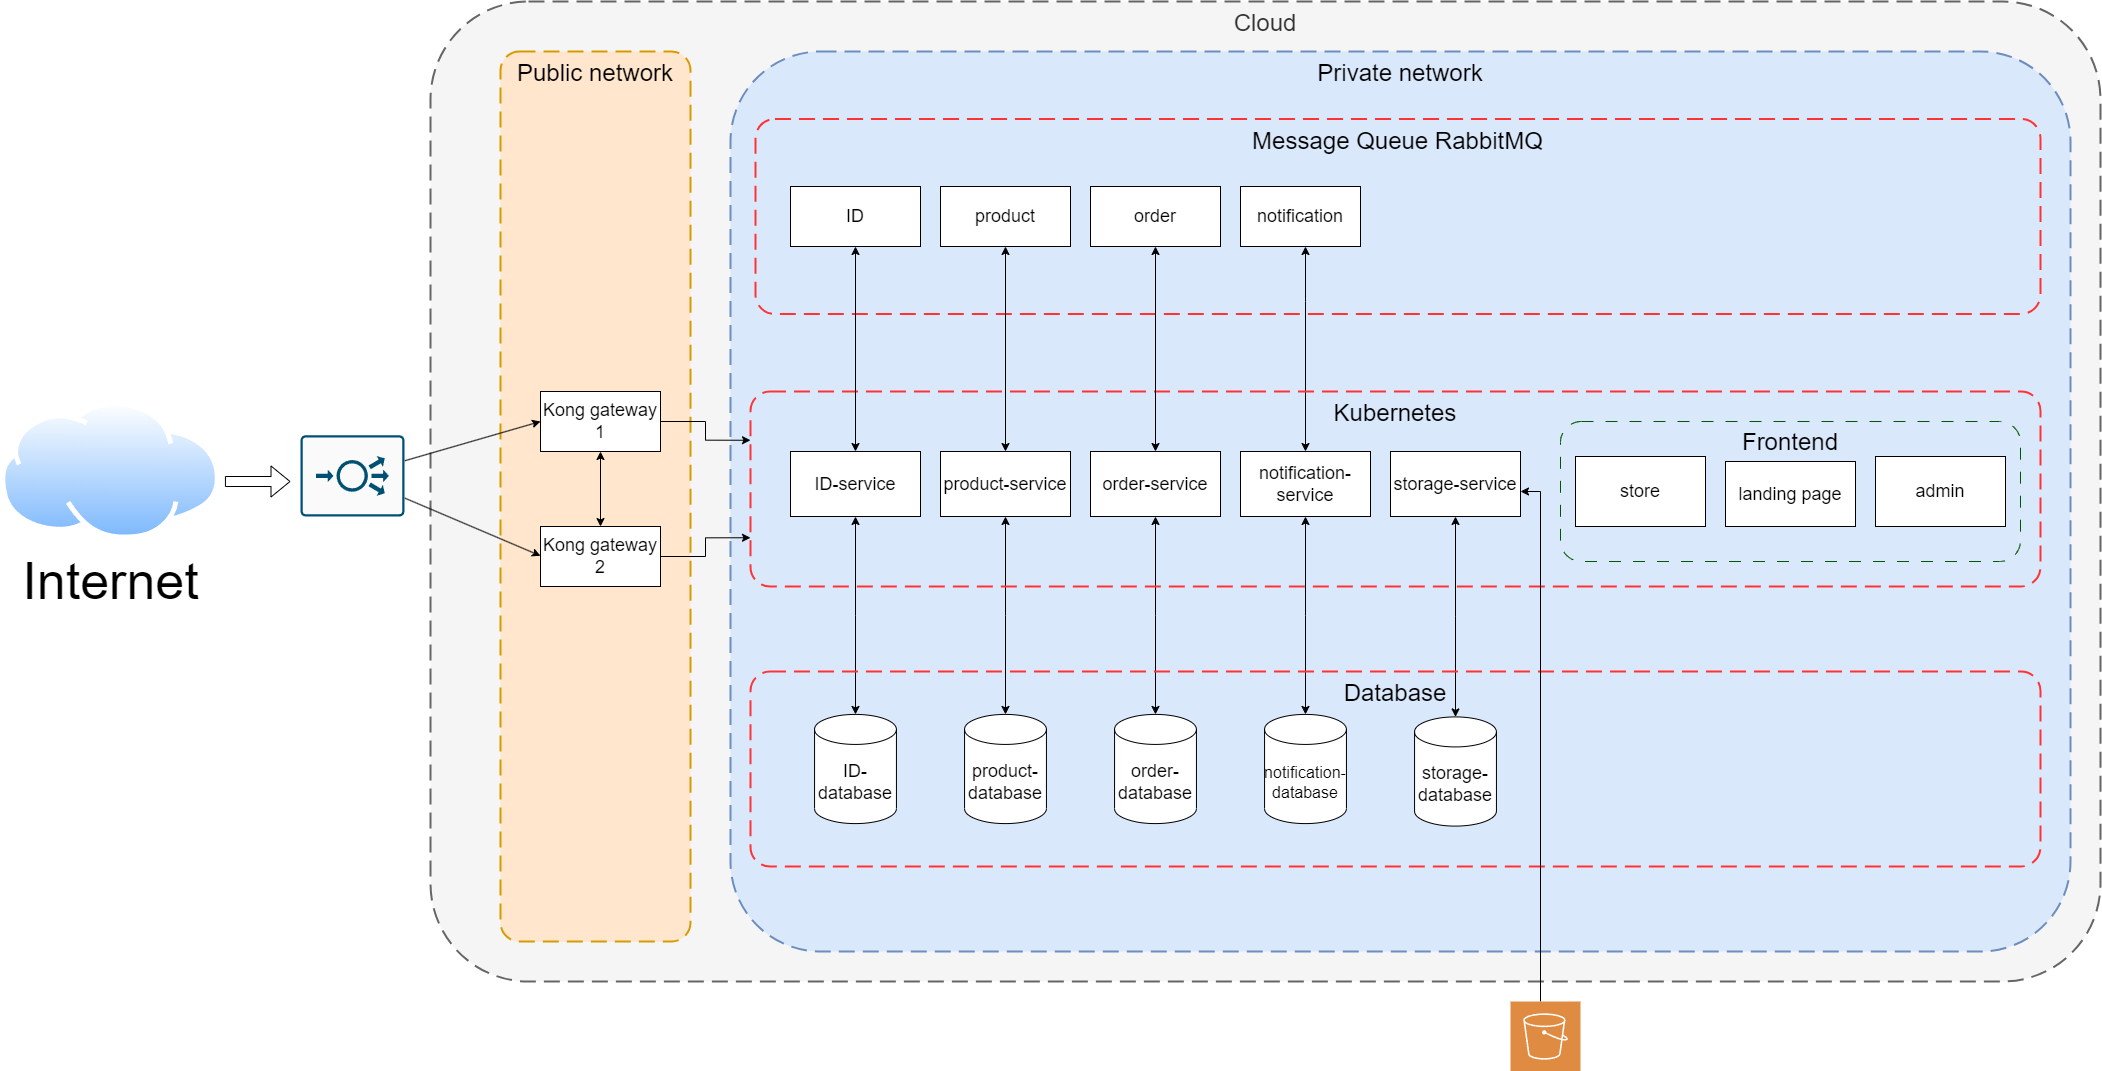
\includegraphics[width=1.1\textwidth]{images/hChip/overall-architecture.png}
	\caption{Hình vẽ mô tả kiến trúc tổng quan của hệ thống quản lý quán ăn}
	\label{fig:overall-architecture}
\end{figure}

Luồng dữ liệu đi vào hệ thống bắt nguồn từ ngoài Internet, nơi tất cả các yêu cầu của người dùng đi qua một GLSB (Global Server Load Balancers).
Ở đây GSLB của hệ thống được triển khai trên Cloudflare giúp phân phối người dùng ở bất cứ nơi nào trên thế giới đến máy chủ khỏe mạnh gần nhất đối với họ.
Điều này sẽ giúp tối ưu hóa thời gian tải trang, giảm thiểu độ trễ, và đảm bảo trải nghiệm truy cập website của người dùng nhanh chóng, mượt mà nhất.

Ngoài ra Cloudflare còn đóng vai trò như một hệ thống phân giải tên miền (DNS).
Khi người dùng truy cập vào trang của hệ thống lần đầu tiên trên trình duyệt web, trình duyệt sẽ gửi truy vấn tới máy chủ DNS cục bộ (resolver), thông thường sẽ là máy chủ của nhà mạng.
Máy chủ DNS cục bộ sẽ kiểm tra liệu tên miền đang được yêu cầu có địa chỉ IP tương ứng không, nếu không tìm thấy máy chủ DNS của nhà mạng sẽ thực hiện một lời gọi khác tới máy chủ DNS tại các cấp cao hơn.
Ở đây cấp độ ngay trên máy chủ cục bộ của nhà mạng sẽ là các máy chủ DNS nơi máy chủ được triển khai như Cloudflare hoặc Google Cloud.
Lời gọi sẽ được chuyển đến DNS của nhà cung cấp mạng của người dùng và sau đó là đến Cloudflare DNS.
Cloudflare sẽ nhận lời gọi của người dùng với tên miền của hệ thống đã được đăng ký trên Namecheap\footnote{https://www.namecheap.com/} và người dùng đến địa chỉ IP (Internet Protocol) của máy chủ phù hợp nhất với người gọi.

Bên trong mỗi máy chủ được triển khai trên Google Cloud sẽ có hai lớp mạng là mạng công cộng được phơi ra ngoài Internet và lớp mạng nội bộ nơi triển khai các thành phần chức năng chính.
Tại lớp mạng công cộng triển khai hai cổng API (API Gateway) phụ trợ cho nhau.
Ngoài những lợi ích chính của một cổng API đó là giúp thống nhất một điểm truy cập đến máy chủ thông qua API Gateway và cải thiện hiệu suất hệ thống nhờ cơ chế cache kết quả truy vấn API cũng như là giới hạn lưu lượng truy cập tránh quá tải, việc sử dụng song song hai cổng API cũng giúp phân phối lưu lượng truy cập giữa các cổng và giúp đảm bảo tính sẵn sàng cao cho hệ thống.

Các cổng API sau đó sẽ chuyển tiếp lời gọi từ ngoài Internet đến hệ thống mạng nội bộ của máy chủ, nơi sẽ triển khai các thành phần chính của mô hình quản lý quán ăn.
Hệ thống ở đây được chia thành ba lớp chính bao gồm lớp hàng đợi tin nhắn sử dụng RabbitMQ, lớp K8s bao gồm các dịch vụ phụ trách xử lý lời gọi của người dùng, và cuối cùng là lớp cơ sở dữ liệu lưu trữ các thông tin quan trọng như dữ liệu của người dùng, nhà hàng, quán ăn, v.v..
Hệ thống được thiết kế theo hướng kiến trúc vi dịch vụ (microservice) tức từng thành phần, chức năng chính của hệ thống sẽ được triển khai và hoạt động trên các môi trường độc lập với nhau giúp hệ thống chịu lỗi tốt hơn, bảo trì dễ dàng, và tiện lợi trong việc nâng cấp, mở rộng sau này.
Mỗi vi dịch vụ microservice có trách nhiệm thực hiện một chức năng cụ thể, ví dụ như dịch vụ thông báo sẽ hoạt động với mục đích duy nhất là nhận thông tin được đẩy đến từ một hoặc nhiều dịch vụ cụ thể và phân phối nó đến với các dịch vụ đã đăng ký nhận thông báo từ các dịch vụ đó.
Việc chia nhỏ hệ thống thành các dịch vụ độc lập mang lại nhiều lợi ích như giúp dễ dàng triển khai và bảo trì cho hệ thống, tăng tính sẵn sàng cũng như là khả năng chịu lỗi, giúp tự động mở rộng hệ thống.
Về mặt phát triển hệ thống, bởi vì mỗi vi dịch vụ đều hoàn toàn độc lập với nhau nên các đội ngũ phát triển của từng chức năng có thể chọn bộ công nghệ phù hợp nhất với nhu cầu và khả năng của đội.

Bằng việc triển khai nền tảng quản lý quán ăn trên Kubernetes (K8s) và Google Cloud Platform (GCP), nhà phát triển sẽ tránh được việc phải cấu hình thủ công cho từng dịch vụ K8s và giảm tải cho quản trị viên hệ thống trong quá trình vận hành và quản lý ứng dụng.
Các ưu điểm công nghệ của K8s sẽ được đề cập rõ hơn trong Mục~\nameref{sec:tehcnologies-used}

Hệ thống cũng sử dụng GCP, một nền tảng dịch vụ điện toán đám mây với gói chức năng đa dạng kèm theo các công cụ hỗ trợ tốt cho hệ thống với kiến trúc vi dịch vụ (microservice) giúp dễ dàng triển khai và vận hành.
Có thể kể đến nền tảng GKE giúp người dùng cấu hình K8s trên GCP một cách dễ dàng, Firebase giúp bảo mật hệ thống, xác thực người dùng truy cập vào hệ thống thông qua việc tạo lập và quản lý tài khoản cả người dùng.
GCP cũng hỗ trợ người sử dụng tránh được các vấn đề liên quan đến cấu hình cơ sở hạ tầng của hệ thống.
Với các tùy chọn đa dạng, người dùng có thể dựa theo nhu cầu thực tế của hệ thống tại từng thời điểm và chọn cấu hình phù hợp.

Tất cả thông tin của người dùng cũng như là nhà hàng, quán ăn tham gia vào nền tảng đều sẽ được lưu trong cơ sở dữ liệu của hệ thống. Các thông tin này có thể là về những lần đặt bàn, thực đơn của quán ăn, những lần gọi món của người dùng, thông tin người dùng, v.v., hoặc thông tin của hệ thống như các chỉ số sức khỏe, các bản ghi hoạt động, v.v.. Nền tảng quản lý quán ăn của khóa luận hiện tại sử dụng MongoDB\footnote{https://www.mongodb.com/}, một cơ sở dữ liệu dạng NoSQL. Chi tiết về cơ sở dữ liệu sẽ được nói rõ hơn trong Mục \autoref{sec:tehcnologies-used}.

\section{Cấu trúc cơ sở dữ liệu} \label{sec:database-design}
Như đã đề cập ở Mục \autoref{sec:tongquan}, pha xây dựng môi trường kiểm thử thực hiện hai nhiệm vụ chính. Nhiệm vụ thứ nhất đó là thực hiện hai tác vụ tiền xử lý mã nguồn. Tác vụ đầu tiên là tác vụ thiết lập môi trường nhằm biên dịch mã nguồn và các ca kiểm thử về sau. Tác vụ này cài đặt các lệnh biên dịch, xác định và liên kết các thư viện mà mã nguồn sử dụng, thiết lập kiểu độ phủ mong muốn cho các đơn vị kiểm thử. Tác vụ thứ hai là tác vụ tạo môi trường tính toán độ phủ. Tác vụ này nhân bản mã nguồn kiểm thử và bổ sung các câu lệnh đánh dấu nhằm phục vụ quá trình xác định các câu lệnh, nhánh được viếng thăm và tính toán độ phủ trong pha sinh dữ liệu kiểm thử tự động. Nhiệm vụ còn lại của pha đó là phân tích mã nguồn kiểm thử và xây dựng đồ thị cấu trúc mã nguồn. Bước phân tích mã nguồn sử dụng công cụ phân tích mã nguồn CDT Parser\footnote{https://github.com/eclipse-cdt/cdt} để trích xuất AST của mã nguồn kiểm thử. Từ thông tin trên AST, phương pháp đề xuất xây dựng đồ thị cấu trúc mã nguồn với các thông tin được phân tích đến mức hàm.

% \subsection*{Đồ thị cấu trúc mã nguồn}
Đồ thị cấu trúc mã nguồn là một cấu trúc dữ liệu biểu diễn mối quan hệ và sự tương tác giữa các thành phần trong mã nguồn kiểm thử. Đồ thị này được biểu diễn bởi một đồ thị có hướng $G = (V, E)$, trong đó $V$ là tập các đỉnh tượng trưng cho các thành phần trong các đơn vị kiểm thử và $E$ là tập các cạnh có hướng nối giữa hai đỉnh tượng trưng cho mối quan hệ phát sinh giữa đỉnh đầu và đỉnh cuối. Mỗi đỉnh trong đồ thị biểu thị cho các đơn vị cơ bản như như tệp mã nguồn, lớp, biến, thư viện được sử dụng, các hàm, v.v. Để làm rõ thể hiện của các hàm thiếu định nghĩa trong đồ thị, khóa luận biểu thị hàm thành hai loại đỉnh hàm: đỉnh nguyên mẫu hàm và đỉnh định nghĩa hàm. Các hàm được khai báo đầy đủ biểu thị bởi đỉnh định nghĩa hàm. Mỗi cạnh trong mã nguồn thuộc một trong các cạnh được mô tả dưới đây.
\begin{itemize}
    \item Cạnh cha con: Thể hiện mối quan hệ cha - con (hay mối quan hệ chứa) giữa hai đơn vị cơ bản trong đơn vị kiểm thử. Ví dụ cho mối quan hệ này có thể kể đến như lớp chứa một số thuộc tính và phương thức, tương đương quan hệ lớp là cha của các thuộc tính và phương thức.
    \item Cạnh Include: Thể hiện mối quan hệ Include giữa hai tệp mã nguồn. Ví dụ cho quan hệ này là dòng lệnh \tcode{\#include} thường thấy trong các mã nguồn C/C++.
    \item Cạnh kế thừa: Thể hiện mối quan hệ kế thừa giữa lớp cha và lớp dẫn xuất. Hai đỉnh của cạnh là hai đỉnh lớp.
    \item Cạnh lời gọi hàm: Thể hiện tương tác giữa hai hàm trong mã nguồn kiểm thử. Hai đỉnh của cạnh là hai đỉnh hàm. Cạnh lời gọi hàm là thành phần quan trọng trong bước xác định các hàm cần tạo stub khi kiểm thử tự động cho một hầm bất kì.
    \item Cạnh định nghĩa: Thể hiện mối quan hệ định nghĩa giữa đỉnh nguyên mẫu hàm ảo và đỉnh định nghĩa hàm ảo. Quan hệ định nghĩa thể hiện nguyên mẫu hàm được trỏ tới tồn tại một khai báo định nghĩa.
\end{itemize}

Đồ thị cấu trúc mã nguồn được xây dựng bằng việc mở rộng từng đỉnh tệp với các cạnh cha con. Quá trình mở rộng đỉnh tệp cấu thành một cây cấu trúc tệp. Tiếp theo, dựa trên các cây cấu trúc tệp, đồ thị cấu trúc mã nguồn được hoàn thiện bằng cách phân tích AST kết hợp tìm kiếm để bổ sung các cạnh quan hệ còn lại. Cạnh định nghĩa là trường hợp đặc biệt được bổ sung sau vào đồ thị trong pha xử lý hàm thiếu định nghĩa.

% \subsection*{Ví dụ về đồ thị cấu trúc mã nguồn}
Hình \autoref{fig:dep-graph} minh hoạ đồ thị cấu trúc mã nguồn của hai tệp mã nguồn a.hpp và a.cpp trong các Đoạn mã \autoref{cod:dep-cpp}, \autoref{cod:dep-hpp}. Trong đó, các cạnh nét liền mũi tên đen thể hiện cạnh cha con giữa hai đỉnh và các kiểu cạnh còn lại được ký hiệu trên hình vẽ với thể hiện tương ứng. Cây cấu trúc mã nguồn của tệp \textit{a.cpp} gồm ba đỉnh hàm. Cây cấu trúc mã nguồn của tệp \textit{a.hpp} gồm hai đỉnh lớp, mỗi đỉnh lớp có quan hệ cha con với một số đỉnh như đỉnh thuộc tính, đỉnh nguyên mẫu hàm. Cạnh Include từ đỉnh tệp \textit{a.cpp} tới đỉnh \textit{a.hpp} tương đương dòng lệnh \tcode{\#include "a.hpp"} trong Đoạn mã \autoref{cod:dep-cpp}. Cạnh lời gọi hàm từ đỉnh định nghĩa hàm \tcode{double A::foo()} tới đỉnh định nghĩa hàm \tcode{int stub()} tương đương lời gọi hàm ở dòng 8 trong tệp \textit{a.cpp}. Đoạn mã ví dụ cho thấy nguyên mẫu hàm ảo \tcode{int func()} trong lớp A có tồn tại định nghĩa bởi hàm \tcode{int A::func()} nhưng đồ thị thiếu cạnh định nghĩa về quan hệ này do cạnh định nghĩa giữa hai đỉnh sẽ được bổ sung sau pha xử lý hàm thiếu định nghĩa.  

\begin{figure}[H]
	\begin{minipage}[t]{0.49\linewidth}
		\begin{lstlisting}[language=C++, caption={Mã nguồn tệp \textit{a.cpp} minh họa đồ thị cấu trúc mã nguồn.}, label={cod:dep-cpp}, captionpos=b]
// a.cpp
#include "a.hpp"
int A::func() {
	/* Function logic */
}
double foo() {
	/* Some logic */
	int ret = stub();
	/* Some logic */
}
int stub() {
	/* Function logic */
}
		\end{lstlisting}
	\end{minipage}
	\begin{minipage}[t]{0.49\linewidth}
		\begin{lstlisting}[language=C++, caption={Mã nguồn tệp \textit{a.hpp} minh họa đồ thị cấu trúc mã nguồn.}, label={cod:dep-hpp}, captionpos=b]
// a.hpp
class IA {
	public: 
	int bar();
};
class A : public IA {
	public:
	A() {}
	int x;
	virtual int beta();
	virtual int func();
	double foo();
}; 
		\end{lstlisting}
	\end{minipage}
			
	\vspace{1cm}
    \includesvg[width=\linewidth]{images/dep-graph}
    \caption{Ví dụ minh hoạ về đồ thị cấu trúc mã nguồn xây dựng trên mã nguồn tệp \textit{a.hpp} và \textit{a.cpp}.}
    \label{fig:dep-graph}
\end{figure}

\section{Giao diện người dùng}\label{sec:UI}
Về tổng quan, phương pháp đề xuất là sự kết hợp giữa phương pháp kiểm thử tượng trưng động~\cite{ConcolicTesting} và phương pháp sinh giả lập mã nguồn tự động~\cite{TUNG2022106821} với các cải tiến trong quá trình xử lý môi trường kiểm thử chứa hàm thiếu định nghĩa và quá trình thực thi tượng trưng lời gọi phương thức. Quá trình kiểm thử tự động bao gồm bốn pha được mô tả trong Hình~\autoref{fig:proposed-flow}. Các pha được in đậm trong hình vẽ thể hiện chúng được bổ sung hoặc cải tiến bởi phương pháp đề xuất.

\begin{figure}[h]
    \centering
    \includesvg[width=\linewidth]{images/proposed-flow}
    \caption{Tổng quan phương pháp đề xuất.}
    \label{fig:proposed-flow}
\end{figure}

Pha đầu tiên trong phương pháp đề xuất là pha xây dựng môi trường kiểm thử. Hai nhiệm vụ chính của pha đó là thực hiện các tác vụ tiền xử lý trên mã nguồn kiểm thử và phân tích mã nguồn để xây dựng đồ thị cấu trúc mã nguồn kiểm thử. Nội dung chi tiết của pha xây dựng môi trường kiểm thử được trình bày trong Mục~\autoref{sec:3-build-env}.

Pha tiếp theo trong phương pháp đề xuất là pha xử lý hàm thiếu nghĩa. Pha này được bổ sung so với phương pháp kiểm thử tự động truyền thống nhằm xử lý các vấn đề phát sinh bởi các hàm thiếu định nghĩa khi kiểm thử tự động cho các mã nguồn chưa hoàn chỉnh. Chi tiết về quá trình xử lý hàm thiếu định nghĩa được mô tả trong Mục~\autoref{sec:handle-undef}.

Sau pha xử lý hàm thiếu định nghĩa, quá trình kiểm thử tự động chuyển sang pha sinh dữ liệu kiểm thử tự động cho các đơn vị kiểm thử. Khóa luận sử dụng phương pháp sinh kế thừa từ phương pháp sinh dữ liệu kiểm thử tượng trưng động và phương pháp sinh giả lập mã nguồn AS4UT (mô tả ở Mục~\autoref{sec:autostub-Lam}). Trong pha sinh dữ liệu kiểm thử tự động, phương pháp đề xuất bổ sung bước sinh giả lập mã nguồn cho các hàm là phương thức của đối tượng nhằm tăng khả năng thực thi các câu lệnh, điều kiện có liên quan đến các đối tượng được sử dụng trong đơn vị kiểm thử. Nội dung chi tiết của pha sinh dữ liệu kiểm thử được trình bày ở Mục~\autoref{sec:autogen}. 

Cuối cùng, các dữ liệu độ phủ được thu thập ở pha sinh dữ liệu kiểm thử được phân tích và tạo thành báo cáo kiểm thử trong pha sinh báo cáo độ phủ mã nguồn. Khóa luận sử dụng công cụ tính độ phủ GNU Coverage - GCOV\footnote{https://gcc.gnu.org/onlinedocs/gcc/Gcov-Intro.html} và công cụ sinh báo cáo độ phủ LCOV để thực hiện nhiệm vụ của pha. Trong đó, GCOV là công cụ phân tích độ phủ tích hợp sẵn trong tập hợp các trình biên dịch GNU (GNU Compiler Collection - GCC), LCOV là một tiện ích mở rộng từ công cụ GCOV với nhiệm vụ sinh báo cáo độ phủ dạng ngôn ngữ siêu văn bản (Hypertext Markup Language - HTML) dựa trên các thông tin độ phủ của GCOV. GCOV và LCOV là hai công cụ có sẵn trong GCC và được sử dụng phổ biến trong các dự án~C/C++ \cite{hu2021software}. Quá trình thực thi ca kiểm thử ở pha trước sinh ra thông tin về số lần chạy qua một dòng, số lần chạy qua các nhánh điều kiện với từng trường hợp đúng, sai theo định dạng của GCOV. Thông tin này sau đó được LCOV tổng hợp, tính toán và đưa ra tệp báo cáo HTML.